\paragraph{nonnative-add}

\subparagraph{Target}
Check the additional relation among three nonnative target objects.

\subparagraph{Constraints logic}
\begin{itemize}
    \item Check equation for gadget: \verb|a + b = c + modular * overflow|;
    \item Check that ``c lt modular''.
\end{itemize}

\subparagraph{Process layout}
See \figref{fig:nonnative-add-layout}.
\begin{figure}[!ht]
    \centering
    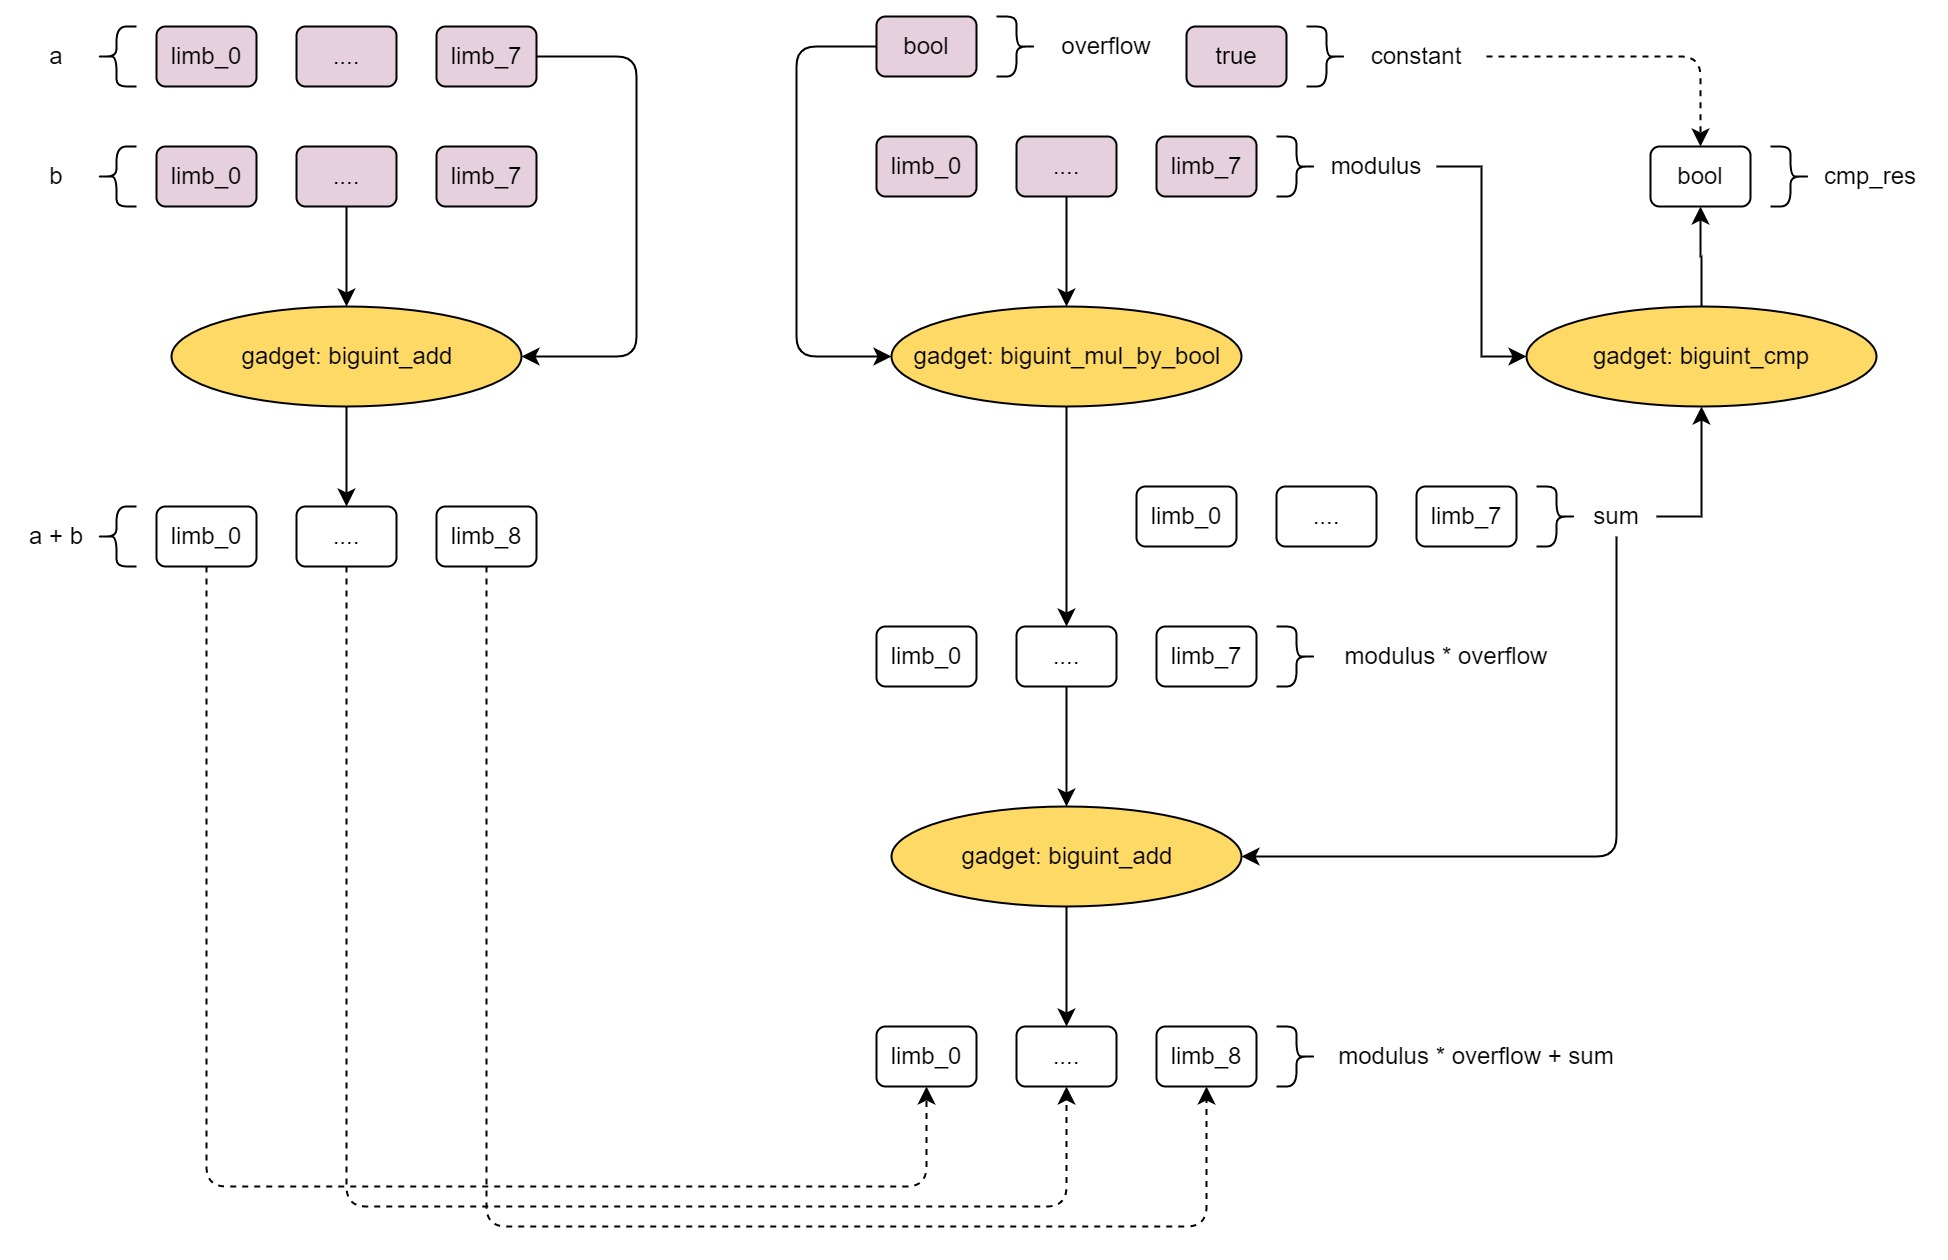
\includegraphics[width=0.8\textwidth]{nonnative-add-layout.jpg}
    \caption{nonnative-add layout}
    \label{fig:nonnative-add-layout}
\end{figure}

\subparagraph{Constraints info and costs}
\begin{itemize}
    \item gadget biguint-add num: 2
    \item gadget biguint-mul-by-bool num: 1
    \item gadget biguint-cmp num: 1
    \item gate type num: 3(U32AddManyGate, ComparisonGate, ArithmeticGate)
    \item gate instance num: 23 = 3(U32AddManyGate) + 16(ComparisonGate) + 2(ArithmeticGate(1,0)) + 1(ArithmeticGate(1,-1)) + 1(ArithmeticGate(1,1))
    \item copy-constraints: 186 = 32 * 2{biguint-add} + 9{biguint-mul-by-bool} + 9 + (4 + 9) * 8{biguint-cmp} = 186
\end{itemize}

\subparagraph{Questions}
\begin{itemize}
    \item When set value to sum?
\end{itemize}
